\section{Architektur des Microservice}
\label{sec: Architektur des Microservice}

\begin{figure}[H]
	\begin{center}
	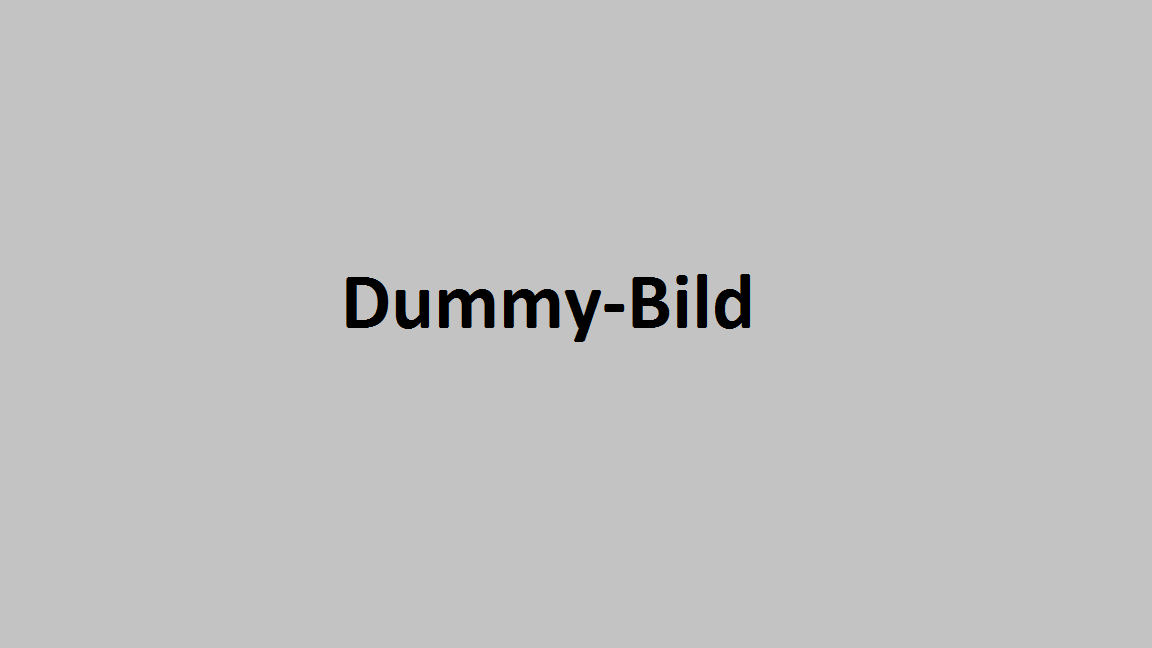
\includegraphics[width=0.65 \textwidth]{./Bilder/dummy.png}
	\end{center}
	\caption{Struktur des Microservice}
	\label{pic:Struktur des Microservice}
\end{figure}


\begin{itemize}
	\item Der Microservice wurde in der Programmiersprache Go\footnote{https:\//golang.org\/doc\/} entwickelt.
	\item \textcolor{red}{ToDo: kurze Beschreibung der Programmstruktur und genauere Beschreibung der Einzelteile in Unterkapiteln}
\end{itemize}

\subsection{Schnittstellen}
\label{subsec: Schnittstellen}

\subsection{Presentation Layer}
\label{subsec: Presentation Layer}

\subsection{Application Layer}
\label{subsec: Application Layer}

\subsection{Persistant Layer}
\label{subsec: Persistant Layer}

\subsection{Integrierte Tests}
\label{subsec: Integrierte Tests}

\subsection{Admin-Frontend}
\label{subsec: Admin-Frontend}

\subsection{Anpassung des Monolithen}
\label{subsec: Anpassung des Monolithen}